\documentclass{beamer}
%
% Choose how your presentation looks.
%
% For more themes, color themes and font themes, see:
% http://deic.uab.es/~iblanes/beamer_gallery/index_by_theme.html
%
\mode<presentation>
{
  \usetheme{default}      % or try Darmstadt, Madrid, Warsaw, ...
  \usecolortheme{crane} % or try albatross, beaver, crane, ...
  \usefonttheme{structurebold}  % or try serif, structurebold, ...
  \setbeamertemplate{navigation symbols}{}
  \setbeamertemplate{caption}[numbered]
} 

\usepackage[english]{babel}
\usepackage[utf8x]{inputenc}

\title[ML]{Machine Learning}
\author{Pawel Wocjan}
\institute{University of Central Florida}
\date{Fall 2020}

\begin{document}

\begin{frame}
  \titlepage
\end{frame}

%%%

\begin{frame}{An Iterative Approach}
\begin{itemize}
    \item The figure below depicts the iterative trial-and-error process that machine learning algorithms use to train a model:
\end{itemize}

\bigskip
\includegraphics[width=\textwidth]{images/GradientDescentDiagram.png}
\end{frame}

%%%

\begin{frame}{Gradient Descent}
\begin{itemize}
\item The iterative approach diagram contains a green box ``compute parameter updates.'' 

\medskip    
\item Let us now discuss the gradient descent algorithm that is used to update the parameters.
\end{itemize}
\end{frame}

%%%

\begin{frame}{Gradient Descent}
\begin{itemize}
\item We consider the linear regression model 

$$\hat{y}=w_1 x_1 + w_2 x_2 + \ldots + w_n x_n b$$

%\item Let us assume that the bias $b=0$ is fixed through the entire training and only $w_1$ can be adjusted.

\item The loss function (mean squared error)

$$\mathcal{L} : \mathbb{R}^{n+1} \rightarrow \mathbb{R}$$ 

depends on the parameters $n+1$ parameters $w_0, w_1, \ldots, w_n$, where $w_0$ is the bias term $b$.

\medskip
\item 
Moreover, $\mathcal{L}$ defines a curve instead of a surface, which simplifies the presentation.
\end{itemize}
\end{frame}

%%%

\begin{frame}{Gradient Decent}
\begin{itemize}
\item For $n=1$, the loss function $\mathcal{L}$ depends on two parameters -- the bias term $b=w_0$ and the weight $w_1$ -- and defines a surface.

\medskip
\item For $n>1$, the loss function $\mathcal{L}$ defines a hypersurface and cannot be visualize so easily.

\medskip
\item To simplify the plots, we assume that $n=1$ and the bias term $b=w_0$ is fixed to be $0$.  Then, the loss function $\mathcal{L}$ defines a curve. 
\end{itemize}
\end{frame}

%%%

\begin{frame}{Gradient Descent}
\begin{itemize}
\item The resulting plot of the loss function $\mathcal{L}$ is be convex. 

\medskip
\item Simply speaking, it means that it is bowl-shaped like this:
\end{itemize}

%\vspace*{-0.5cm}
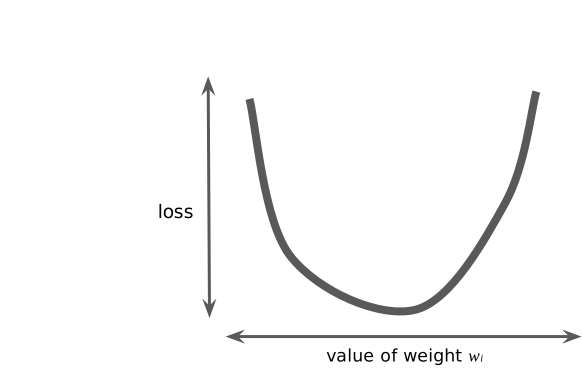
\includegraphics[width=0.9\textwidth]{images/convex.png}
\end{frame}

%%%

\begin{frame}{Gradient Descent}
\begin{itemize}
\item It turns out that even in the general case the loss function $\mathcal{L}$ is convex.

\medskip
\item This is important because problems have only one minimum.

\medskip    
\item Calculating the loss function for all parameter values $w_0,\ldots,w_n\in\mathbb{R}^{n+1}$ set would be an inefficient way of finding the minimum.

\medskip    
\item Let's examine a better mechanism -- very popular in machine learning -- called {\bf gradient descent}.
\end{itemize}
\end{frame}

%%%

\begin{frame}{Gradient Descent}
\begin{itemize}
\item The first stage in gradient descent is to pick a starting value. 

\medskip
\item The starting point doesn't matter much; therefore, many algorithms simply set $w_i=0$ or set the $w_i$ to random values.
\end{itemize}

\includegraphics[width=0.9\textwidth]{images/GradientDescentStartingPoint.png}
\end{frame}

%%%

\begin{frame}{Gradient Descent}
\begin{itemize}
\item The gradient descent algorithm then calculates the gradient of the loss function $\mathcal{L}$ at the starting point. 

\medskip
\item The gradient 

$$\nabla\mathcal{L}\in\mathbb{R}^{n+1}$$ 

is a vector whose entries 

$$(\nabla\mathcal{L})_i$$ 

are given by the partial derivatives 

$$\partial \mathcal{L}/\partial w_i$$ 

of the loss function $\mathcal{L}$ with respect to the weights $w_i$.
\end{itemize}
\end{frame}

%%%

\begin{frame}{Gradient Descent}
\begin{itemize}
\medskip    
\item The $\nabla\mathcal{L}$ gradient has both a direction and a magnitude.

\medskip    
\item The gradient points which way is ``warmer'' or ``colder.'' 

\medskip
\item The gradient always points in the direction of steepest increase in the loss function. 

\medskip 
\medskip For the case $n=1$ and the bias $w_0=b$ is fixed to be $0$, the gradient of the loss function $\mathcal{L}$ is simply the slope of the curve $\mathcal{L}$, that is, the derivative with respect to $w_1$.
\end{itemize}
\end{frame}


%%%

\begin{frame}{Gradient Descent}
\begin{itemize}
\item The gradient descent algorithm takes a step in the direction of the negative gradient $-\nabla \mathcal{L}$ to reduce the loss.
\end{itemize}

\vspace{0.1cm}
\includegraphics[width=0.9\textwidth]{images/GradientDescentNegativeGradient.png}
\end{frame}

%%%

\begin{frame}{Gradient Descent}
\begin{itemize}
\item More precisely, the gradient descent algorithm updates the starting point as follows:

\vspace{-0.25cm}

$$ \boldsymbol{w} \leftarrow \boldsymbol{w} - \alpha \nabla\mathcal{L} $$

where $\alpha$ is the learning rate.
\end{itemize}
\includegraphics[width=0.9\textwidth]{images/GradientDescentGradientStep.png}
\end{frame}

%%%

\begin{frame}{Key Terms}
\begin{itemize}
    \item gradient
    \item gradient descent
    \item step
\end{itemize}
\end{frame}


\subsection{Learning Rate}

\begin{frame}{Learning Rate}
\begin{itemize}
\item The gradient vector has both a direction and a magnitude. 

\medskip
\item The gradient descent algorithm multiplies the gradient by a scalar known as the learning rate (also sometimes called step size) to determine the next point. 

\medskip
\item For example, if the gradient magnitude is $2.5$ and the learning rate is $0.01$, then the gradient descent algorithm will pick the next point $0.025$ away from the previous point.
\end{itemize}
\end{frame}

%%%

\begin{frame}{Learning Rate}
\begin{itemize}
\item The learning rate is a so-called {\bf hyperparameter}. 

\medskip
\item A hyperparameter is a parameter that is external to the model.
\end{itemize}
\end{frame}

%%%

\begin{frame}{Learning Rate}
\begin{itemize}
\item If the learning rate that is too small, learning will take too long:
\end{itemize}
\includegraphics[width=0.9\textwidth]{images/LearningRateTooSmall.png}
\end{frame}


%%%

\begin{frame}{Learning Rate}
\begin{itemize}
\item If the learning rate is too large, the next point will perpetually bounce haphazardly across the bottom of the well:
\end{itemize}
\includegraphics[width=0.9\textwidth]{images/LearningRateTooLarge.png}
\end{frame}

%%%

\begin{frame}{Learning Rate}
\begin{itemize}
\item There's a Goldilocks learning rate for every linear regression problem.
\end{itemize}
\includegraphics[width=0.9\textwidth]{images/LearningRateJustRight.png}
\end{frame}

%%%

\begin{frame}{Key Terms}
\begin{itemize}
\item hyperparameter
\item learning rate
\item step size
\end{itemize}
\end{frame}

\begin{frame}{Stochastic Gradient Descent}

%%%

\begin{itemize}
\item In gradient descent, a {\bf batch} is the total number of examples you use to calculate the gradient in a single iteration. 
    \item So far, we've assumed that the batch has been the entire data set. 
    \item But often data sets contain huge numbers of examples with huge numbers of features.
    \item Consequently, a batch can be enormous. A very large batch may cause even a single iteration to take a very long time to compute.
    \item A large data set with randomly sampled examples probably contains redundant data. In fact, redundancy becomes more likely as the batch size grows. 
    \item Some redundancy can be useful to smooth out noisy gradients, but enormous batches tend not to carry much more predictive value than large batches.
\end{itemize}
\end{frame}

\begin{frame}{Stochastic Gradient Descent}

\begin{itemize}
\item What if we could get the right gradient on average for much less computation? 

\medskip
\item By choosing examples at random from our data set, we could estimate (albeit, noisily) a big average from a much smaller one. 

\medskip
\item {\bf Stochastic gradient descent (SGD)} takes this idea to the extreme--it uses only a single example (a batch size of 1) per iteration. 

\medskip
\item Given enough iterations, SGD works but is very noisy. The term ``stochastic'' indicates that the one example comprising each batch is chosen at random.
\end{itemize}

\end{frame}

\begin{frame}{Reducing Loss}
\begin{itemize}
    \item {\bf Mini-batch stochastic gradient descent (mini-batch SGD)} is a compromise between full-batch iteration and SGD. A mini-batch is typically between $10$ and $1,000$ examples, chosen at random. 
    
\medskip
\item Mini-batch SGD reduces the amount of noise in SGD but is still more efficient than full-batch.
\end{itemize}
\end{frame}

\begin{frame}{Key Terms}
\begin{itemize}
    \item batch
    \item batch size
    \item mini-batch
    \item stochastic gradient descent (SGD)
\end{itemize}

\end{frame}

\end{document}